%%%%%%%%%%%%%%%%%%%%%%%%%%%%%%%%%%%%%%%%%%%%%%%%%%%%%%%%%%%%%%%%%%%%%%%%%%%
%%%                                                                     %%%
%%%   LaTeX template voor het verslag van P&O: Computerwetenschappen.   %%%
%%%                                                                     %%%
%%%   Opties:                                                           %%%
%%%     tt      Tussentijdsverslag                                      %%%
%%%     eind    Eindverslag                                             %%%
%%%                                                                     %%%
%%%   3 oktober 2016                                   %%%
%%%   Versie 1.4                                                        %%%
%%%                                                                     %%%
%%%%%%%%%%%%%%%%%%%%%%%%%%%%%%%%%%%%%%%%%%%%%%%%%%%%%%%%%%%%%%%%%%%%%%%%%%%

\documentclass[eind]{Setup/penoverslag}
\usepackage{url}
\usepackage{amsmath}
\usepackage{caption}
\usepackage{subcaption}
\usepackage{amsmath,bm}
\usepackage{pdfpages}
\usepackage{gensymb}
\usepackage{float}
\usepackage[dutch]{babel}

%%% PACKAGES %%%


\begin{document}

% == TITELPAGINA == %
\team{Zilver}
\year{2016-2017}
\members{Bram Vandendriessche (Co\"ordinator)\\
         Arne Vlietinck (Secretaris)\\
         Matthias Van der Heyden \\
         Jef Versyck\\
         Vincent Vliegen\\
         Laura Vranken}
\maketitlepage


% == SAMENVATTING == %
\begin{abstract}
\noindent
{\em Auteur: Arne Vlietinck}\\
\\
Dit verslag behandelt het ontwerp en de implementatie van een Autopilot en Virtual Testbed voor een drone. In de simulator is voor de eerste mijlpaal een rode bol in een witte ruimte te zien. Bij de tweede mijlpaal wordt deze wereld uitgebreid met een windkracht in een willekeurige richting. Voor de derde mijlpaal zijn er verschillende bollen zichtbaar die allemaal op een zo efficiënt mogelijke manier moeten worden doorprikt. Bij de laatste mijlpaal zijn niet alle bollen direct zichtbaar. Een uitbreiding is het ontwijken van grijze obstakels.
\\
De Autopilot zorgt voor een correcte aansturing van de drone. Hij bepaalt de vliegroute op basis van informatie verkregen van twee camera's die zich op de drone bevinden. Hierbij is de relatieve plaatsbepaling van de bol ten opzichte van de drone van belang. De Autopilot leidt daaruit de beweging van de drone af en laat de simulator deze uitvoeren.
\\
Het programma wordt interactief gemaakt door het gebruik van \textit{GUI's}. Deze geven de mogelijkheid het camerastandpunt te kiezen, extra bollen toe te voegen, ook de voltooiingsgraad, snelheid en positie van de drone worden weergegeven. Daarnaast kunnen externe factoren (wind en gravitatieconstante) aangepast worden.
\end{abstract}


% == INHOUDSOPGAVE == %
\tableofcontents\newpage

% == INLEIDING == %
\section*{Inleiding}
\label{sec: Inleiding}
% \emph{[In de inleiding schets je de context, probleemstelling en doelstellingen van het project.  Je kunt ook kort aangeven wat er wel en niet in het verslag staat (bij een tussentijds verslag).]} 
{\em Auteurs: Laura Vranken \& Arne Vlietinck}
\\\\
\noindent
Drones zijn de laatste jaren enorm in populariteit toegenomen en blijven hierdoor ook in positieve zin evolueren. Ze worden tegenwoordig gebruikt voor talloze toepassingen. De bekendste toepassing bevindt zich binnen Defensie, die drones gebruiken om informatie te verkrijgen over vijandelijk gebied zonder mensenlevens te moeten riskeren. Daarnaast hebben ook grote bedrijven (o.a. Amazon\footnote{Amazon Prime Air}) de weg naar deze technologie gevonden. De toekomst brengt echter nog veel meer voordelen. Enkele voorbeelden  \cite{website:microdrones} zijn veiligheidsinspectie van windturbines of elektriciteitslijnen, luchtsteun bij zoek- en reddingsoperaties, bewaking en luchtfotografie.
\\
Wanneer een drone autonoom functioneert, is een betrouwbare aansturing door de Autopilot van levensbelang. Hij moet namelijk bestand zijn tegen allerlei externe factoren (bv. wind, obstakels...).
\\
\\
Dit verslag behandelt de autonome aansturing van een drone, meer bepaald een quadcopter, en is een vervolg op het tussentijds verslag \cite{arcticle:tssnTijds}. Er wordt uitgegaan van een drone waarop twee voorwaarts gerichte camera's bevestigd zijn. Op basis van deze beelden moeten afstand en positie tegenover het doel ingeschat worden en nieuwe bewegingsopdrachten voor de drone gegenereerd worden. Deze bewegingen worden weergegeven in een Virtual Testbed \cite{arcticle:opgavePeno}. Dit is een softwaresysteem dat een fysieke opstelling van een drone en camera's simuleert. De simulator genereert beelden van de drone uit verschillende standpunten a.d.h.v. de verkregen bewegingsopdrachten van de Autopilot. 
\\
\\
De Autopilot en Virtual Testbed moeten zo ontworpen worden dat de drone in staat is om zijn doel, een niet grijze bol, te lokaliseren en ernaar toe te vliegen. Dit eventueel onder lichte invloed van wind in willekeurige richtingen. Bovendien moet ook voor beiden een grafische user interface (\textit{GUI}) ontworpen worden. De \textit{GUI} toont de vooruitgang en laat de gebruiker toe allerlei informatie (snelheid, positie en verschillende camerastandpunten) op te vragen. Daarnaast kan de gebruiker nieuwe bollen toevoegen en de wind manueel aanpassen in de verschillende richtingen. 
\\
\\
De tekst is als volgt opgebouwd. %TODO


%Eerst wordt het ontwerp van de Autopilot en Virtual Testbed verder uitgediept (sectie \ref{sec:Ontwerp}). Vervolgens wordt er ingegaan op de gebruikte algoritmen (sectie \ref{sec:Algoritmes}) en wordt de opbouw van onze software verduidelijkt (sectie \ref{sec:Software}). Ook is er extra informatie te vinden over de \textit{GUI} (sectie \ref{sec:GUI}). Er wordt afgesloten met de uitgevoerde testen te bespreken (sectie \ref{sec:Testen}) en een kort besluit. \\
\newpage

% == Testbed == %
\section{Testbed}
\label{sec: Testbed}
\subsection{Polyhedra en het bestaande ontwerp}
\noindent {\em Auteur: Bram Vandendriessche}
\\\\
\noindent Het ontwerp van de simulator dat vorig semester tot stand kwam, zorgde ervoor dat de uitbreiding ervan met polyhedra vrij eenvoudig in te voeren was. Door een nieuw type \textit{Polyhedron} dat erft van \textit{WorldObjects}, moesten er in \textit{World} zelf slechts enkele extra methodes ge\"implementeerd worden m.b.t. het toevoegen en verwijderen van een \textit{Polyhedron} aan de bestaande wereld.\\
\\
\noindent 
Een \textit{Polyhedron} zelf is zo ontworpen dat die bestaat uit verschillende \textit{Triangles}. De \texttt{draw()}-methode van de \textit{Polyhedron} draagt elke \textit{Triangle} die tot de Polyhedron behoort, op om zichzelf te tekenen. Een \textit{Triangle} bestaat uit co\"ordinaten voor zijn drie hoekpunten en een kleur voor het buitenste gedeelte van de driehoek. Op basis daarvan worden de binnenste hoekpunten berekend en wordt er een kleur afgeleid uit de kleur van de buitenste driehoek zodat de driehoek voldoet aan de gegeven beperkingen m.b.t. de kleur, zie Tabel \ref{table: HSVwaarden}, en de oppervlakte.\\
\\
\noindent
Het ontwerp van het Testbed heeft de grote zwakte dat het erg moeilijk is om individuele elementen en methodes zoals bijvoorbeeld \textit{Collision Detection}, te testen. Dit komt doordat de objecten erg afhankelijk zijn van de wereld waarin ze bestaan. Die wereld is bovendien altijd afhankelijk van de \textit{gl}-component van \textit{OpenGL}, waardoor het noodzakelijk is een volledige \textit{GL}-wereld op te zetten voor de test kan worden uitgevoerd. Een oplossing hiervoor zou zijn om de objecten en wereld zo op te splitsen dat presentatie en representatie gesplitst worden, zodat het representatie-gedeelte onafhankelijk kan gebruikt worden. Daarnaast zou dan enkel de wereld weet moeten hebben van haar objecten en niet andersom, zodat objecten onafhankelijk van de wereld kunnen worden getest. Deze inzichten werden dan ook toegepast bij het ontwerp van de 3D-component van de Autopilot (zie \ref{sec: 3dAutopilotScan}).\\
\\
\noindent
Voor het testen van de Autopilot zijn verschillende figuren ontworpen. Zij vallen onder \textit{PredefinedPolyhedron}, een subklasse van \textit{Polyhedron} die ook een positie mee kan krijgen bij creatie. Hierdoor kan de figuur naar een gewenste positie worden geplaatst. De gewone Polyhedron (dus de niet vooraf gedefinieerde) krijgen geen 3D-co\"ordinaat mee. Hun positie wordt gezet op het massapunt van de polyhedron, i.e. de gemiddelde 3D-co\"ordinaat van alle hoekpunten. Op die manier wordt gezorgd dat de positie logisch is t.o.v. de hoekpunten. Het is dus niet mogelijk dat de driehoeken van een figuur bijvoorbeeld rond (20,0,0) gedefinieerd worden, maar de polyehdron zelf een positie van (0,0,-40) krijgt toegewezen. De figuren vari\"eren van een eenvoudige piramide met vier hoekpunten tot meer complexe figuren zoals een kubus met een opening in, waarbij de Autopilot zal moeten weten dat het voor de drone niet mogelijk is hierdoor te vliegen, zie Figuur \ref{fig: polyhedra}.

\begin{figure}[H]
	\centering
	\begin{subfigure}{.5\textwidth}
		\centering
		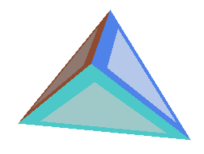
\includegraphics[width=.4\linewidth]{Testbed/4point.png}
		\caption{Eenvoudige figuur}
	\end{subfigure}%
	\begin{subfigure}{.5\textwidth}
		\centering
		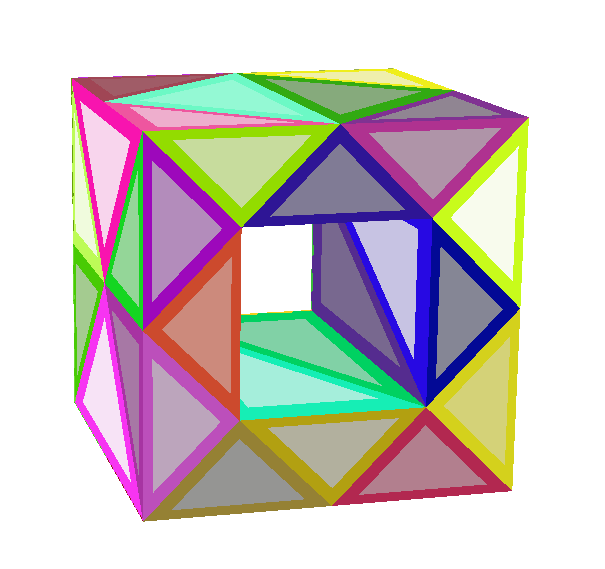
\includegraphics[width=.4\linewidth]{Testbed/poly2.png}
		\caption{Complexere figuur}
	\end{subfigure}
	\caption{Voorgedefinieerde polyhedra.}
	\label{fig: polyhedra}
\end{figure}

\label{sec:polyhedraTestbed}
\newpage
\subsection{Collision Detection}
\noindent {\em Auteur: Jef Versyck}
\\\\
Aangezien polyhedra niet per definitie mooie cirkels zijn zoals de bollen voordien, moet \textit{Collision Detection} aangepast worden. Eerst wordt er vergeleken of de afstand tussen de twee centra van de objecten (een polyhedron en de drone) kleiner is dan beide hun radii opgeteld. De radius van een polyhedron wordt gedefinieerd als de grootste afstand tussen het centrum van de polyhedra en zijn punten. \\
\noindent
Vervolgens wordt er getest of de loodrechte afstand op het vlak van een \textit{Triangle} vanuit het middelpunt van de drone kleiner is dan de straal van de drone. Hierbij wordt het vlak waarin de \textit{Triangle} zich bevindt, berekend aan de hand van het kruisproduct van twee vectoren van de \textit{Triangle} en een hoekpunt ervan. Nadien wordt de loodrechte projectie op het vlak bepaald. Dit punt heet P. In formulevorm: 
\begin{gather*}
	a\cdot x + b\cdot y + c\cdot z = d \\ 
	t = -\frac{a \cdot x_{drone} + b \cdot y_{drone} + c \cdot z_{drone} - d}{a^2 + b^2 + c^2}  \\ P =
	\begin{Bmatrix}
	a\cdot t + x_{drone}\\ 
	b\cdot t + y_{drone}\\ 
	c\cdot t + z_{drone}
	\end{Bmatrix}
\end{gather*}

\noindent
 Dit is echter niet genoeg. De loodrechte projectie van het massacentrum  kan zich buiten de \textit{Triangle} bevinden en zo een foutief resultaat geven. Om te zien of het punt zich binnen de \textit{Triangle} bevindt, wordt de methode van de barycentrische coördinaten \cite{website:barycentric-coordinates} gehanteerd. Het principe hierachter is dat elk punt P in de driehoek geschreven kan worden als een lineaire combinatie van de hoekpunten (A, B en C) van een driehoek. De som van alle co\"effici\"enten moet gelijk zijn aan één en alle co\"effici\"enten moeten groter zijn dan nul. In formulevorm:
 
 \begin{gather*}
 	P = u\cdot A + v\cdot B + w\cdot C \\
 	0 \le u,v,w \le 1 \\
 	u + v + w = 1
 \end{gather*}
\noindent
Er is echter een probleem met deze methode, namelijk dat de berekening van de \textit{Collision Detection} aangeeft dat er geen botsing was gebeurd, terwijl dit in de werkelijkheid wel zo was. \\
Dit komt door een randgeval waarin de drone vlak naast de \textit{faces} (de driehoeken) van een polyhedron vliegt. De loodrechte projectie op het vlak van de \textit{face} zou zich dan niet in de driehoek bevinden, wat dus zegt dat er geen botsing is gebeurd volgens de \textit{Collision Detection}, terwijl een rand van de drone wel de \textit{face} aanraakt. Het randgeval doet zich echter weinig voor en wanneer het zich voordoet, wordt het vrijwel direct opgelost. Immers, de drone heeft een snelheid naar de polyhedron waardoor hij de projectie zo zal verplaatsen dat deze zich uiteindelijk wel in de driehoek bevindt. Er zal dus bijgevolg toch een botsing optreden. Figuur \ref{fig:CollisionDetectionProbleem} toont een voorbeeld van dit probleem.

\begin{figure}[H]
	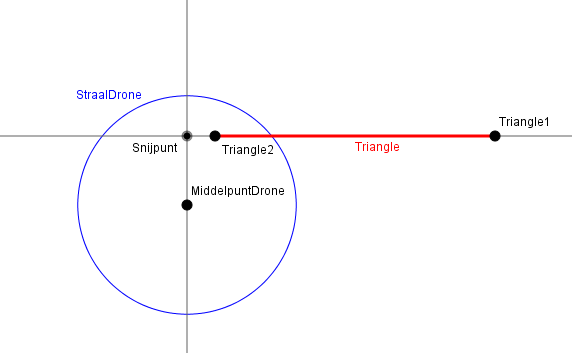
\includegraphics[width=1\textwidth]{Testbed/CollisionDetectionProbleem.png}
	\caption{Probleem met Collision Detection.\\ }
	\label{fig:CollisionDetectionProbleem}
\end{figure}
\subsection{Generator en editor}
\noindent {\em Auteur: Jef Versyck}
\\\\
Ook werd er dit semester gevraagd om zelf een wereld-generator te implementeren. Elk bestand gegenereerd door deze generator, moet voldoen aan de opgestelde eisen. Op dit moment zijn er twee generators: één die een wereld met bollen maakt uit het vorige semester en één die een wereld met polyhedra genereert. Deze laatste kiest uit verschillende vooraf aangemaakte \textit{PredefinedPolyedra}, zoals vermeld in Sectie \ref{sec:polyhedraTestbed}.
\\

\noindent
Daarnaast is de editor meer gedetailleerd uitgewerkt. Men selecteert eerst een object met de muis. Met behulp van de toetsen i en k (bewegen volgens positieve en negatieve x-as), j en l (bewegen volgens positieve en negatieve z-as), u en o (bewegen volgens positieve en negatieve y-as), kan het aangeklikte object verplaatst worden in de wereld. Ook kunnen er zowel gewone als obstakel-polyhedra toegevoegd worden via de \textit{GUI's} op een gekozen positie in de ruimte. Ten slotte is er ook nog een mogelijkheid om polyhedra te verwijderen door ze te selecteren en de DELETE knop te gebruiken. 
\\\\
\noindent
Verder is er nog een nieuwe methode aangemaakt die gebruikt zal worden bij het scannen. Deze methode zorgt ervoor dat de drone op een onnatuurlijke wijze rond een polyhedron vliegt. De drone maakt drie cirkels in het xz-vlak, telkens op verschillende y-waarden, zodat hij de hele figuur kan zien. Dit is niet mogelijk in werkelijkheid, aangezien de drone naar de figuur blijft kijken en zich nooit roteert om te bewegen in het xz-vlak met een pitch of roll.



% == AP == %
\newpage
\section{Autopilot}
\label{sec: Autopilot}
\subsection{Vliegstrategie}
\noindent {\em Auteur: Vincent Vliegen}
\\
\\
De drone start altijd met een gegeven positie en ori\"entatie. Afhankelijk van de missie moeten de positie en ori\"entatie veranderen. De Autopilot bepaalt de nodige thrust en rotatiesnelheden om in de gewenste situatie terecht te komen. 
\\
\\
Omwille van de uitwendige krachten op de drone, vliegt de drone niet enkel in de richting van de thrustkracht. Aan de hand van de gewenste verplaatsingsrichting en de huidige snelheid, wordt de versnellingsrichting van de drone berekend. Deze richting is dezelfde als de som van de krachten, bestaande uit de zwaartekracht, drag, wind en thrust. De thrustgrootte wordt zo gekozen dat de drone zo goed mogelijk in de richting van het doel vliegt.
\\
\\
Daarna wordt een gewenste ori\"entatie berekend. Afhankelijk van de afstand tot de gewenste positie en de snelheid naar deze positie, bepaalt de Autopilot aan welke versnelling de drone moet versnellen of vertragen. Zo kan ook hier de gewenste thrustrichting afgeleid worden in functie van de bewegingsvergelijking en het krachtenevenwicht.
\\
\\
\noindent
Indien er een gewenste kijkrichting is, zal de Autopilot voorzien dat de drone zo goed mogelijk gericht staat in deze richting. Dit is bijvoorbeeld nuttig bij het scannen. Anderzijds, wanneer de kijkrichting niet uitmaakt, wordt een ori\"entatie bepaald met kijkrichting gericht op de doelpositie.\\
\\
\noindent
Om polyhedra te doorprikken, wordt eerst gekeken of er doelen zichtbaar zijn. Indien dit niet het geval is, wordt ernaar gezocht, anders wordt van elk object dat gezien wordt, een punt bijgehouden en de bijhorende (zichtbare) kleuren van dat object. Van alle objecten die gezien werden, wordt het dichtste punt gezocht en als doel ingesteld. Wanneer de drone dicht bij het object komt, worden de camerabeelden opnieuw geanalyseerd. Er wordt dan gekeken of een van de kleuren die bij het doel-punt hoorde, zichtbaar is. Indien dit niet het geval is, wordt aangenomen dat het object reeds doorprikt is. Een foute assumptie is ineffici\"ent, maar geen ramp gezien het object later opnieuw zal worden opgemerkt. In het andere geval, waarbij de kleur nog steeds zichtbaar is, worden eventuele andere kleuren toegevoegd aan het object en de doelpositie wordt nauwkeuriger ingesteld. \\
\\
\noindent
Na het doorprikken van een object (of in de foute assumptie dat het object doorprikt is), zal het volgende dichtste object als doel worden ingesteld. Indien er geen doelen meer zichtbaar zijn, wordt opnieuw gezocht naar mogelijke doelen. %TODO: klopt dit?
\subsection{Rotaties}
\noindent {\em Auteurs: Vincent Vliegen \& Arne Vlietinck}
\\\\
Wanneer de gewenste ori\"entatie bekend is, kunnen de nodige rotatiesnelheden berekend worden om de drone bij te sturen. Aan de hand van projecties toegepast op de kijkvector, berekent de Autopilot twee mogelijke yaw- en pitch-waarden die wanneer de rotaties worden uitgevoerd, de drone laten kijken volgens de gewenste kijkrichting. Ook komen twee mogelijke waarden voor de roll voort uit projecties toegepast op de thrustvector. De Autopilot kiest de waarden die er voor zorgen dat de drone niet over kop gaat.
\\
De drone heeft maximale rotatiesnelheden. Indien de yaw te groot is om tijdens \'e\'en tijdsinterval uit te voeren, moeten de pitch- en roll-waarden herberekend worden. Dit gebeurt opdat de thrustvector de juiste ori\"entatie zou aannemen.\\
Om de rotaties te berekenen wordt gebruik gemaakt van de Rodrigues'\cite{website:Rodrigues} rotatie formules.
\begin{equation} \label{eq: Rodrigues}
v_{rot} = v \cos(\theta) + (k \times v) \sin(\theta) + k(k \cdot v)(1-\cos(\theta))
\end{equation}
In Formule \ref{eq: Rodrigues} is \(v\) een drie dimensionele vector, \(k\) een eenheidsvector die de rotatieas weergeeft en \(\theta\) de hoek volgens de rechterhandregel. Aan de hand van deze formule is het dus mogelijk om een vector \(v\) te roteren rond een as \(k\) met een bepaalde hoek \(\theta\).\\
Er is gebruik gemaakt van deze formule om de drone zo realistisch mogelijke rotaties te laten uitvoeren, waarbij de gevraagde rotaties ook werkelijk worden uitgevoerd. Als voorbeeld op dit principe wordt er een pitch van \(10\degree\) doorgegeven. Dan zal de drone effectief \(10\degree\) verder pitchen rond zijn eigen pitch-as en niet rond een vast gedefinieerd assenstelsel ergens in de ruimte.
\label{sec: Rotaties}
\subsection{Obstakels}
\noindent {\em Auteur: Arne Vlietinck}
\\\\
Obstakels vermijden is noodzakelijk om als Autopilot een goede werking te garanderen. Om te controleren of er zich al dan niet een obstakel op de route van de drone bevindt, gaat de Autopilot als volgt te werk:\\
Ten eerste wordt er een bol gedefinieerd rond de driehoek. Deze bol is de kleinst mogelijke bol die alle drie de hoekpunten bevat. Bij deze bol wordt wel een veiligheidsmarge gerekend van anderhalf keer de breedte van de drone. Dit om bij onvoorziene afwijkingen van de drone toch het obstakel met zekerheid te ontwijken. Vervolgens wordt er gecontroleerd of de bol gesneden wordt door het pad van de drone. Indien dit niet het geval is, zal er geen object in de weg liggen en kan de drone het kortste pad nemen richting zijn doel. Is dit echter wel het geval, dan zou het kortste pad leiden tot het crashen van de drone. Daarom wordt er een tijdelijk doel gedefinieerd dat buiten deze cirkel, maar wel zo goed mogelijk op het pad tussen de drone en het doel ligt. Het is dan de bedoeling dat de drone eerst naar de tussenstop vliegt om zo op een veilige manier voorbij het obstakel te geraken. Deze methode wordt ge\"illustreerd door Figuur \ref{fig:obstakel}. Wanneer deze actie geslaagd is, kan de drone zijn weg naar het einddoel voortzetten.
\begin{figure}[H]
\centering
	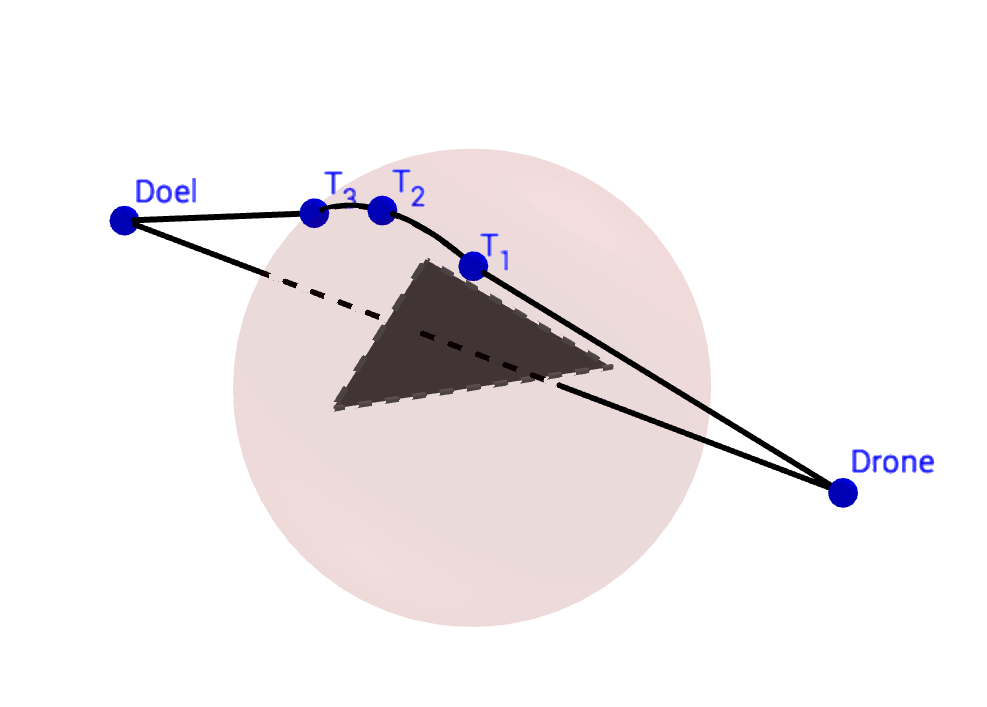
\includegraphics[width=0.6\textwidth]{AP/Obstakel.png}
	\caption{Methode om een obstakel te ontwijken. \(T_1, T_2\) en \(T_3\) stellen tussenstops voor.}
    \label{fig:obstakel}
\end{figure}
\subsection{Windcorrectie}
\noindent {\em Auteur: Vincent Vliegen}
\\
\\
Wind zal zorgen voor een verandering van de positie en ori\"entatie van de drone.  Aangezien de Autopilot wordt opgeroepen met een constant tijdsinterval, kunnen er voorspellingen worden gemaakt over de ruimtelijke situering van de drone, wanneer er een bepaalde hoeveelheid tijd is verlopen.
\\\\
De Autopilot stelt de thrust en rotatiesnelheden in. Met behulp van de uitwendige krachten en rotaties kunnen de verplaatsingsrichting en verandering van ori\"entatie bepaald worden. Wanneer ook het constante tijdsinterval in rekening wordt gebracht, kan de verwachte positie benaderd worden aan de hand van de bewegingsvergelijking (zie Tabel \ref{table: uitlegFormule} voor uitleg van de symbolen):
\begin{equation}
	 \frac{(\vec{T} + \vec{G} + \vec{D} + \vec{W}) }{2m} * (\Delta t)^2 + \vec{v_0} * \Delta t + \vec{x_0} = \vec{x}_{exp}
\end{equation}
De verwachte ori\"entatie wordt bepaald door het huidige assenstelsel van de drone te roteren met de drie nieuw berekende rotatierates. Dit resulteert in de ori\"entatie van de drone in het volgende frame, moest er geen invloed van de wind zijn.
\\
\\
De Autopilot controleert in het begin van elke cyclus of de verwachte positie en de eigenlijke positie overeenkomen, respectievelijk de verwachte en eigenlijke ori\"entatie. Zo niet, is de afwijking te verklaren als een verandering van de windtranslatie en -rotatie. Het verschil in positie is het gevolg van een onnauwkeurige benadering van de windtranslatie. Deze kan gecorrigeerd worden door de kracht te berekenen die de afwijking heeft veroorzaakt, en dan op te tellen bij de huidige windkracht.
\begin{equation}
	\frac{(\vec{W}_{corr}) }{2m} * (\Delta t)^2 = \vec{x}-\vec{x}_{exp}
\end{equation}
De afwijking in ori\"entatie is te wijten aan een windrotatie. De windrotaties worden uitgevoerd rond het wereldassenstelsel, dat vast is en niet mee roteert. Op basis van de rotatiematrix van de wind, kunnen de X, Y en Z rotaties worden afgeleid, die het verwachtte assenstelsel corrigeren naar het nieuwe assenstelsel. 
\begin{table}[H]
	\centering
	\begin{tabular}{ l|l }
		\(\vec{T}\): Thrust & \(\Delta t\): tijdsverschil tussen twee frames\\
		\(\vec{G}\): Gravity & \(\vec{v_0}\): startsnelheid\\
		\(\vec{D}\): Drag & \(\vec{x_0}\): beginpositie\\
		\(\vec{W}\): Wind & \(\vec{x}_{exp}\): verwachte positie\\
		\(\vec{W}_{corr}\): Windcorrectie & \(m\): massa drone \\
	\end{tabular}
	\caption{\label{table: uitlegFormule}Verduidelijking van de gebruikte notaties.}
\end{table}

% == Scannen == %
\section{Scannen}
\label{sec: scannen}
\subsection{Beeldverwerking}
\noindent {\em Auteur: Laura Vranken}
\\\\
\noindent
Om polyhedra te kunnen scannen, moet de drone ze eerst herkennen op de ontvangen afbeeldingen. 
Hiervoor worden eerst alle pixels gegroepeerd per kleur. Dan worden de kleuren opgesplitst in verschillende lijsten volgens hun soort, nl. binnen- en buitendriehoek van respectievelijk target en obstakel. Zie Tabel \ref{table: HSVwaarden} voor de exacte voorwaarden.
\begin{table}[H]
	\centering
\begin{tabular}{ l | c | c | c }
	 & H & S & V\\\hline
	Buitendriehoek target & ? & \(>\) 0.55 & \(>\) 0.55 \\
	Binnendriehoek target & ? & \(<\) 0.45 & \(>\) 0.55 \\
	Buitendriehoek obstakel & ? & \(>\) 0.55 & \(<\) 0.45 \\
	Binnendriehoek obstakel & ? & \(<\) 0.45 & \(<\) 0.45\\
\end{tabular}
\caption{\label{table: HSVwaarden}Combinatie HSV-waarden om de verschillende driehoeken te herkennen. Hue-waarde mag willekeurig gekozen worden.}
\end{table}
\noindent Om een driehoek te kunnen tekenen, zijn de drie hoekpunten vereist. Deze hoeken zijn bepaald door de buitenste pixels en worden berekend door een rechthoek rond de driehoek te tekenen. Aangezien het kan zijn dat twee hoekpunten op dezelfde hoogte of breedte liggen, worden twee pixels, de minimum en maximum pixel, van elke zijde van de rechthoek bepaald. Figuur \ref{fig:DrieGevallenDriehoeken}a geeft een voorbeeld weer van deze methode. Op deze manier worden acht pixels gevonden. Natuurlijk heeft een driehoek geen acht hoeken, dus worden de overeenkomstige buitenste pixels samengenomen tot één hoekpunt. 
\\\\
Een volledige driehoek behoudt drie hoekpunten. Ook een driehoek die evenwijdig met een zijde door een andere polyhedron of door de rand van het beeld afgesneden wordt, kan drie hoekpunten overhouden. Indien er niet evenwijdig met een zijde is afgesneden, blijven er vier of meer hoekpunten over. Zie Figuur \ref{fig:DrieGevallenDriehoeken}b voor het eerste geval en Figuur \ref{fig:DrieGevallenDriehoeken}c voor het tweede geval. De figuren met meer dan drie hoekpunten worden niet meer bekeken; ze zijn niet volledig.
\\\\
Om onderscheid te maken tussen volledige en afgesneden driehoeken met drie hoekpunten, wordt de buitendriehoek samen met de overeenkomstige binnendriehoek verder onderzocht. Indien hun zwaartepunten samenvallen, zijn ze volledig. Indien ze niet matchen, kan geconcludeerd worden dat een deel van de driehoek is weggevallen. Zwaartepunten kunnen bepaald worden door Formule \ref{formule: zwaartepunt}: \begin{equation}
\label{formule: zwaartepunt}
(x_{zpt},y_{zpt}) = ( \ \frac{1}{3}(x_1 + x_2 + x_3) , \ \frac{1}{3}(y_1 + y_2 + y_3) \ )
\end{equation}
\\
Dit gebeurt voor beide camera's en vervolgens worden de gevonden hoekpunten gecombineerd en doorgestuurd naar de fysische component van de Autopilot om omgezet te worden naar 3D-co\"ordinaten in het wereldassenstelsel. Uit deze re\"ele hoekpunten kunnen dan later de driehoeken getekend worden.
\\
\begin{figure}[H]
	\centering
	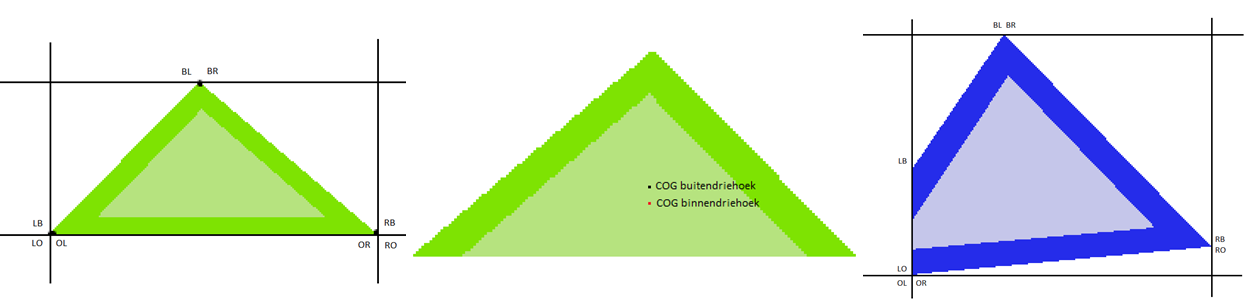
\includegraphics[width=1\textwidth]{Scannen/BeeldverwerkingDriehoeken.png}
	\caption{Bepalen van de buitenste acht punten van mogelijke driehoeken. \\ a) Een volledige driehoek. \\ b) Evenwijdig afgesneden driehoek met drie hoekpunten. De zwaartepunten (COG) liggen echter op een andere plaats. \\ c) Willekeurig afgesneden driehoek met vier hoekpunten. \\ 
	Afkortingen: LO = links onder, LB = links boven, RO = rechts onder, RB = rechts boven, OL = onder links, OR = onder rechts, BL = boven links, BR = boven rechts.}
	\label{fig:DrieGevallenDriehoeken}
\end{figure}
\subsection{3D-voorstelling}
\noindent {\em Auteurs: Bram Vandendriessche \& Matthias Van der Heyden}
\\\\
Voor de grafische weergave van de gescande objecten, is een andere aanpak gehanteerd dan bij de \textit{Polyhedra} in het Testbed. Hierdoor is er een onderscheid verkregen tussen presentatie (visueel) en interne representatie. 
Een \textit{Polyhedron} is in twee delen opgesplitst: een data-object (\textit{PolyhedronAPData}) dat de hoekpunten en kleuren bevat en een grafische component die de driehoeken van de \textit{Polyhedron} tekent. Net als het Testbed werkt ook de Autopilot met een \textit{World}, die voor de implementatie van de \textit{OpenGL}-functies zorgt. De wereld is opgesplitst in een data-object en een grafisch object (\textit{WorldAPVisual}). Dit laatste zal met de gegevens uit de data-wereld een visuele voorstelling kunnen verzorgen.\\
\\
\noindent
De \textit{Polyhedra} worden gekarakteriseerd door hun driehoeken en die op hun beurt door hoekpunten en kleuren. Er werd daarom een type \textit{CustomColor} toegevoegd dat de binnen- en buitenkleur van \'e\'en driehoek voorstelt. Deze \textit{CustomColors} worden toegewezen aan \textit{Points}, die de hoekpunten van de driehoeken voorstellen. Elk \textit{Point} heeft een 3D-co\"ordinaat en bevat verschillende \textit{CustomColors}, naargelang het aantal driehoeken waartoe het punt behoort. Aangrenzende driehoeken zullen immers een of twee punten gemeenschappelijk hebben. \\
\\
\noindent
Voor dit concept bevat de interne representatie een \textit{HashMap} die \textit{CustomColors} op basis van de buitenste kleur van een driehoek mapt naar een lijst van drie \textit{Points}. Op deze manier kan \textit{PolyhedronAPDrawer} heel eenvoudig de driehoeken tekenen per kleur, dus per driehoek gezien elke \textit{CustomColor} uniek is. Voor aangrenzende driehoeken zal de \textit{HashMap} dan van deze kleuren mappen naar lijsten waarin dit punt steeds voor komt.
\noindent
Het voordeel van de \textit{Points} is dat er geen drie afzonderlijke punten per driehoek worden bijgehouden, waardoor bij verschuiving van een hoekpunt van een driehoek, alle driehoeken die dit punt bevatten automatisch worden aangepast. Op deze manier blijft de figuur steeds mooi gesloten.
\label{sec: 3dAutopilotScan}
\subsection{Van camerabeelden naar 3D-figuur}
\noindent {\em Auteur: Matthias Van der Heyden}\\
\noindent
\\
Indien de missie \textit{ScanObject} is geselecteerd, vraagt deze bij elke oproep van \texttt{timeHasPassed()} de co\"{o}rdinaten van de figuren die de drone op dat moment kan zien, op aan de beeldverwerking. Driehoeken met een kleur die nog niet eerder werd gezien, worden toegevoegd aan de \textit{PolyhedronAPData} die op dat moment onder constructie is. Hiervoor worden nieuwe \textit{Points} aangemaakt waaraan de kleur van de driehoek wordt toegevoegd. Deze kleur wordt vervolgens samen met de drie punten in de \textit{HashMap} geplaatst. Alvorens \textit{Points} toe te voegen, wordt eerst op basis van de co\"{o}rdinaten gecontroleerd of dit punt niet reeds bestond. Indien dit het geval is, wordt slechts de kleur toegevoegd aan het \textit{Point} waarna de \textit{Hashmap} voor de kleur dit \textit{Point} zal bevatten.\\
Wanneer de driehoek reeds tot de \textit{PolyhedronAPData} behoorde, worden de co\"{o}rdinaten van het \textit{Point} aangepast naar een gewogen gemiddelde van de oorspronkelijke waarde en de nieuwe metingen. Op deze manier wordt geprobeerd om de co\"{o}rdinaten naar een nauwkeurige benadering te laten convergeren naarmate meer data verzameld wordt.
\subsection{Vliegstrategie}
\noindent {\em Auteur: Laura Vranken}
\\\\
\noindent
Vliegen rond een polyhedron om deze te kunnen scannen, vereist een zekere strategie. Ten eerste moet het mogelijk zijn om alle vlakken van het object te bekijken. Vervolgens moet bepaald worden wanneer de drone de volledige polyhedron heeft gezien en kan stoppen met deze te scannen. Ten slotte moet hij verschillende polyhedra van elkaar kunnen onderscheiden.
\\
Door een tekort aan tijd en onverwachte vertragingen is het laatste punt niet uitgewerkt. Het vervolg van deze paragraaf gaat dus enkel verder in op het scannen van één polyhedron.
Hoewel deze strategie volledig uitgewerkt is, wordt tijdens de demo gevlogen op basis van een op voorhand ingestelde baan van het Testbed. Dit doordat het huidige vliegen van de Autopilot nog niet nauwkeurig genoeg is om gecontroleerd rond een polyhedron te vliegen.
\\\\
Er wordt gestart vanuit het beginbeeld met de polyhedron recht voor de drone. Elke zichtbare driehoek wordt gesplitst in zijn drie zijdes en deze worden in een lijst bijgehouden. Aangrenzende driehoeken delen altijd eenzelfde zijde. Wanneer dus beide driehoeken van een zijde herkend zijn, kan deze zijde uit de lijst verwijderd worden en als gezien geklasseerd worden. Als deze lijst leeg is, kan vervolgens besloten worden dat beide driehoeken van elke zijde gescand zijn en dat de polyhedron volledig afgewerkt is.
\\\\
Om volledig rond de polyhedron te kunnen vliegen, wordt telkens bepaald uit de lijst welke zijde nog een driehoek mist. De voorkeur gaat uit naar een zijde die het dichtst in de buurt van de drone ligt en zal dus degene zijn die het laatst is toegevoegd. Het doel is te vliegen naar een bepaalde positie waaruit die zijde en zijn aanliggende driehoeken kunnen waargenomen worden. Die positie wordt door het volgende algoritme bepaald.
\\
Eerst wordt een rechte getrokken tussen de drone en het zwaartepunt van de gekende driehoek. Vervolgens wordt er op die rechte een punt gekozen dat iets verder ligt dan de driehoek. Het is een schatting van het centrumpunt van de polyhedron. Vervolgens wordt een nieuwe rechte getrokken vanuit dit centrumpunt door het middelpunt van de te bekijken zijde. Hierop wordt opnieuw een punt gedefinieerd, dit keer op een afstand van 1 meter van de polyhedron. Dat punt is de nieuwe volgende positie naar waar gevlogen moet worden. Het algoritme wordt ge\"illustreerd in Figuur \ref{fig:ScanFly}.
\\
\begin{figure}[H]
\centering
	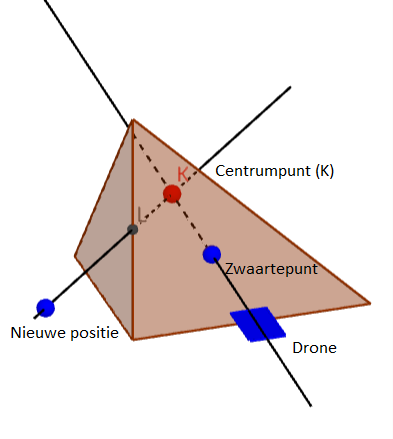
\includegraphics[width=0.4\textwidth]{Scannen/FigStrategieScan.png}
	\caption{Bepalen van de nieuwe positie om de zijde en aanliggende driehoek te zien.}
    \label{fig:ScanFly}
\end{figure}

% == Testen == %
\section{Testen}
\label{sec: Testen}
%[{\em Beschrijf de tests die je uitgevoerd hebt om de correcte werking en de nauwkeurigheid van je software te bepalen.  Geef de resultaten op compacte en heldere manier weer, bv. met tabellen of grafieken.  Denk na over de beste manier om de resultaten weer te geven.  Ze moeten je conclusies ondersteunen.  Formuleer de conclusies.}]\\

\noindent {\em Auteurs: Arne Vlietinck; redactie: Arne Vlietinck}
\\
\\
Voor beide programma's worden er uitvoerig testklasses gegenereerd en uitgevoerd. Hiermee kan de correcte werking en de nauwkeurigheid van de gebruikte algoritmes gecontroleerd worden. Ook eventuele programmeerfouten komen aan het licht en kunnen op deze manier aangepast worden. 
\\
Naar gelang de milestones uitdagender worden, zullen de testklassen striktere en hogere eisen stellen aan de ge\"implementeerde tests.


% == Algemeen Resultaat == %
\section{Algemeen Resultaat}
\label{sec: AlgemeenResultaat}
\noindent {\em Auteurs: Arne Vlietinck \& Jef Versyck; redactie: Arne Vlietinck}
\\
\\
Om dit project tot een goed einde te brengen werd gedurende het geheel een planning voor ogen gehouden. Deze werd zo goed mogelijk gevolgd en up to date gehouden. Beide gantt charts kunnen gevonden worden in Appendix \ref{App: AppendixPlanning}.
\\
Op het moment van schrijven raakt de drone de dichtstbijzijnde bol met zekerheid. Vervolgens vliegt hij in cirkels rond zijn tweede doelwit. Dit doordat er een snelheidscomponent is in een andere richting dan het doel van de drone. Na verloop van tijd slaagt de drone er meestal in om de tweede bol te doorprikken. Indien er wind wordt toegevoegd, kan de drone met veel minder zekerheid naar de bollen toe vliegen. 



% == BESLUIT == %
\section*{Besluit}
\label{sec: Besluit}
\noindent {\em Auteurs: Arne Vlietinck; redactie: Arne Vlietinck}
\\
\\
Dit verslag rapporteert het cre\"eren van een drone Virtual Testbed en zijn Autopilot. De Autopilot berekent de juiste instructies a.d.h.v. de dronecamera's. Via deze beelden slaagt de Autopilot erin om de drone de eerste bol te laten doorprikken. Van groot belang om dit geheel te laten werken, is een juiste visualisatie door de simulator. Daarnaast moeten alle bewegingen in juist volgorde uitgevoerd worden op zowel de drone als camera's. Zoals er beschreven staat in de mijlpalen werd er ook een variabele windfactor ge\"implementeerd. Wanneer de wind van toepassing is, is het halen van de mijlpalen niet altijd mogelijk. 
\\ 
Daarnaast worden de vele keuzes die tijdens het project gemaakt werden, verdedigd in bovenstaande secties.
\\
Tijdens het programmeren werd een duidelijk schema voor ogen gehouden zodanig dat uitbreidingen voor eventueel volgende mijlpalen vlot kan verlopen.\\

% == REFERENTIES == %
\bibliographystyle{siam}
\bibliography{references}


% == APPENDICES == %
\newpage
\appendix
\section{Planning}
\label{app: Planning}
\subsection{Gantt chart deel 1} 
	\begin{figure}[H]
		\begin{center}
			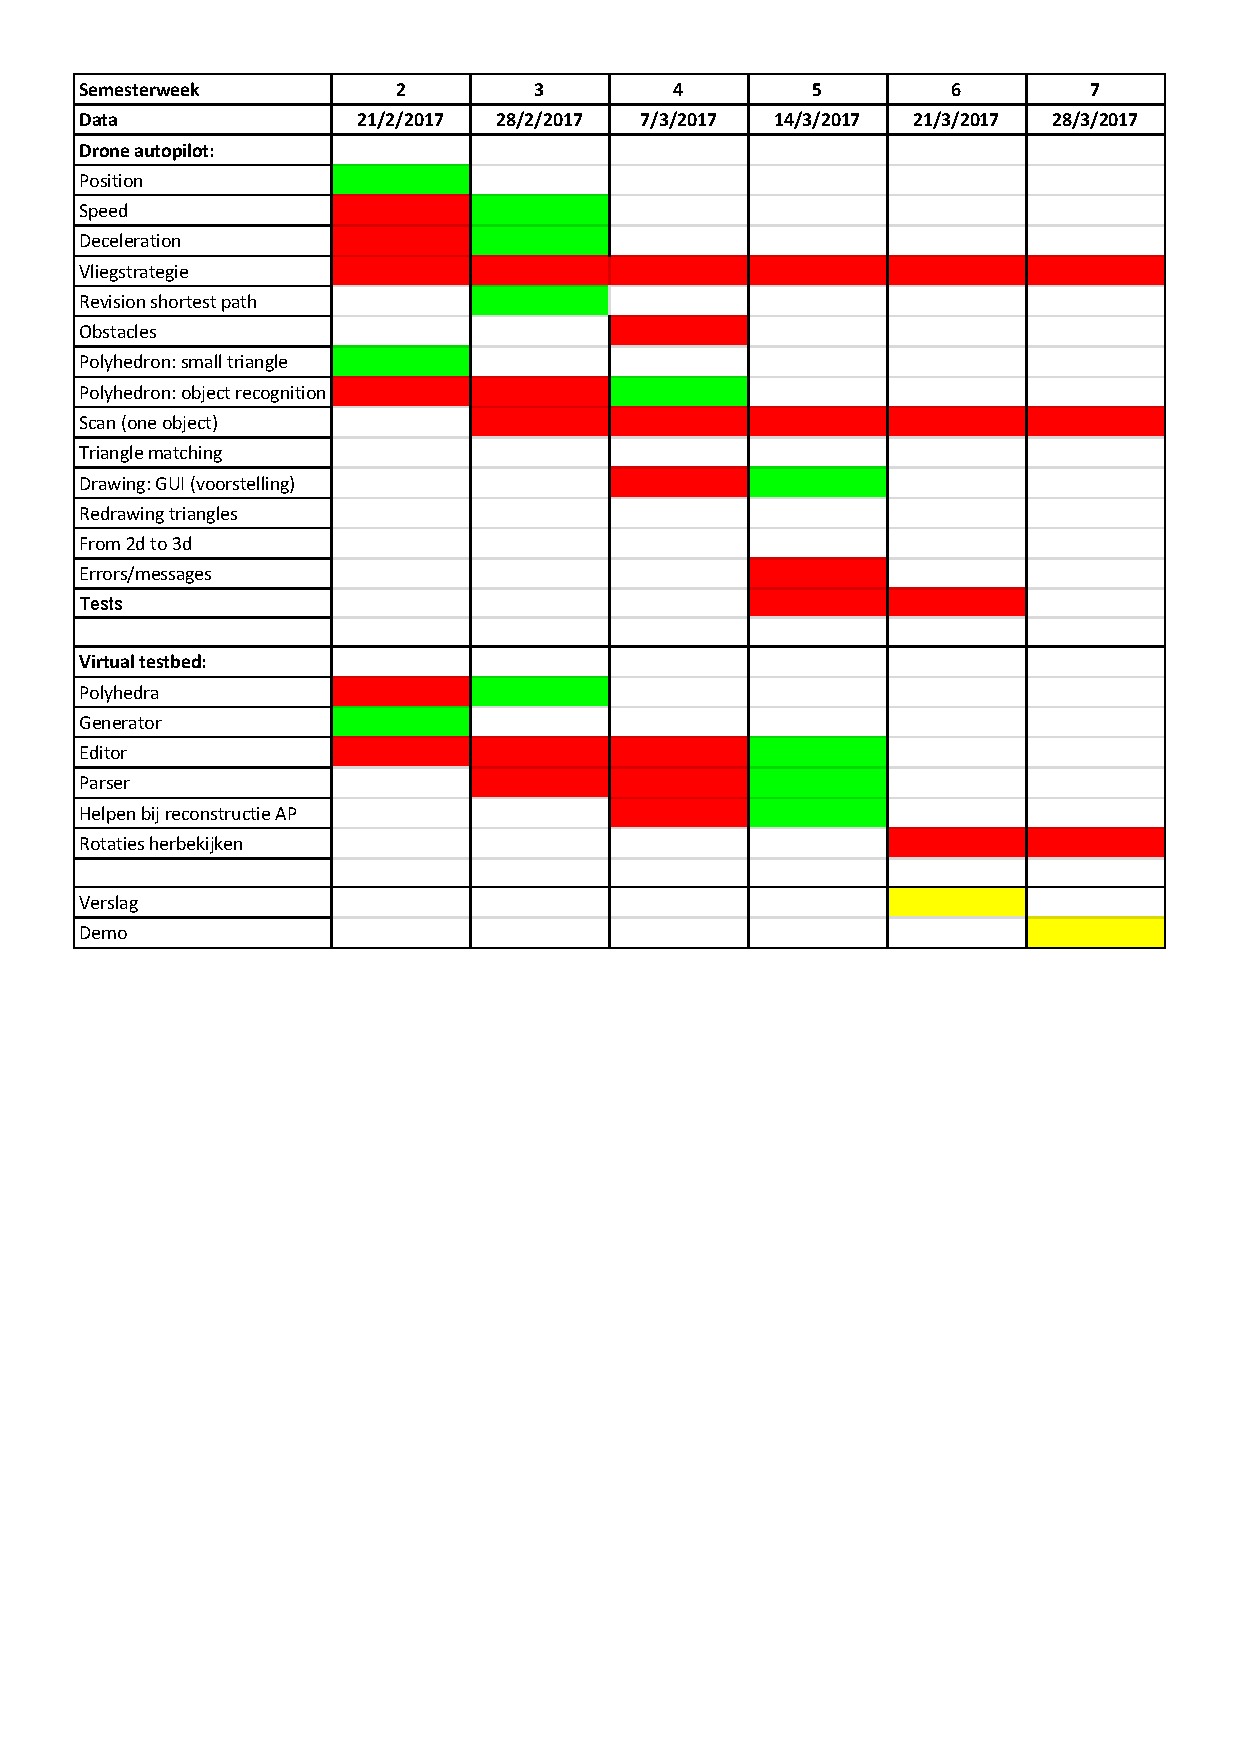
\includegraphics[scale=0.60]{Appendices/Planning_Deel1.pdf}
		\end{center}
		\caption{Deze Gantt chart geeft de planning gedetailleerd weer van het eerste deel. De verschillende delen van de mijlpalen worden opgesplitst om een gedetailleerde taakverdeling te kunnen maken. Voltooide onderdelen worden in het groen aangeduid, de deadlines in het geel.}
	\end{figure}
\subsection{Gantt chart deel 2} 
	\begin{figure}[H]
		\begin{center}
			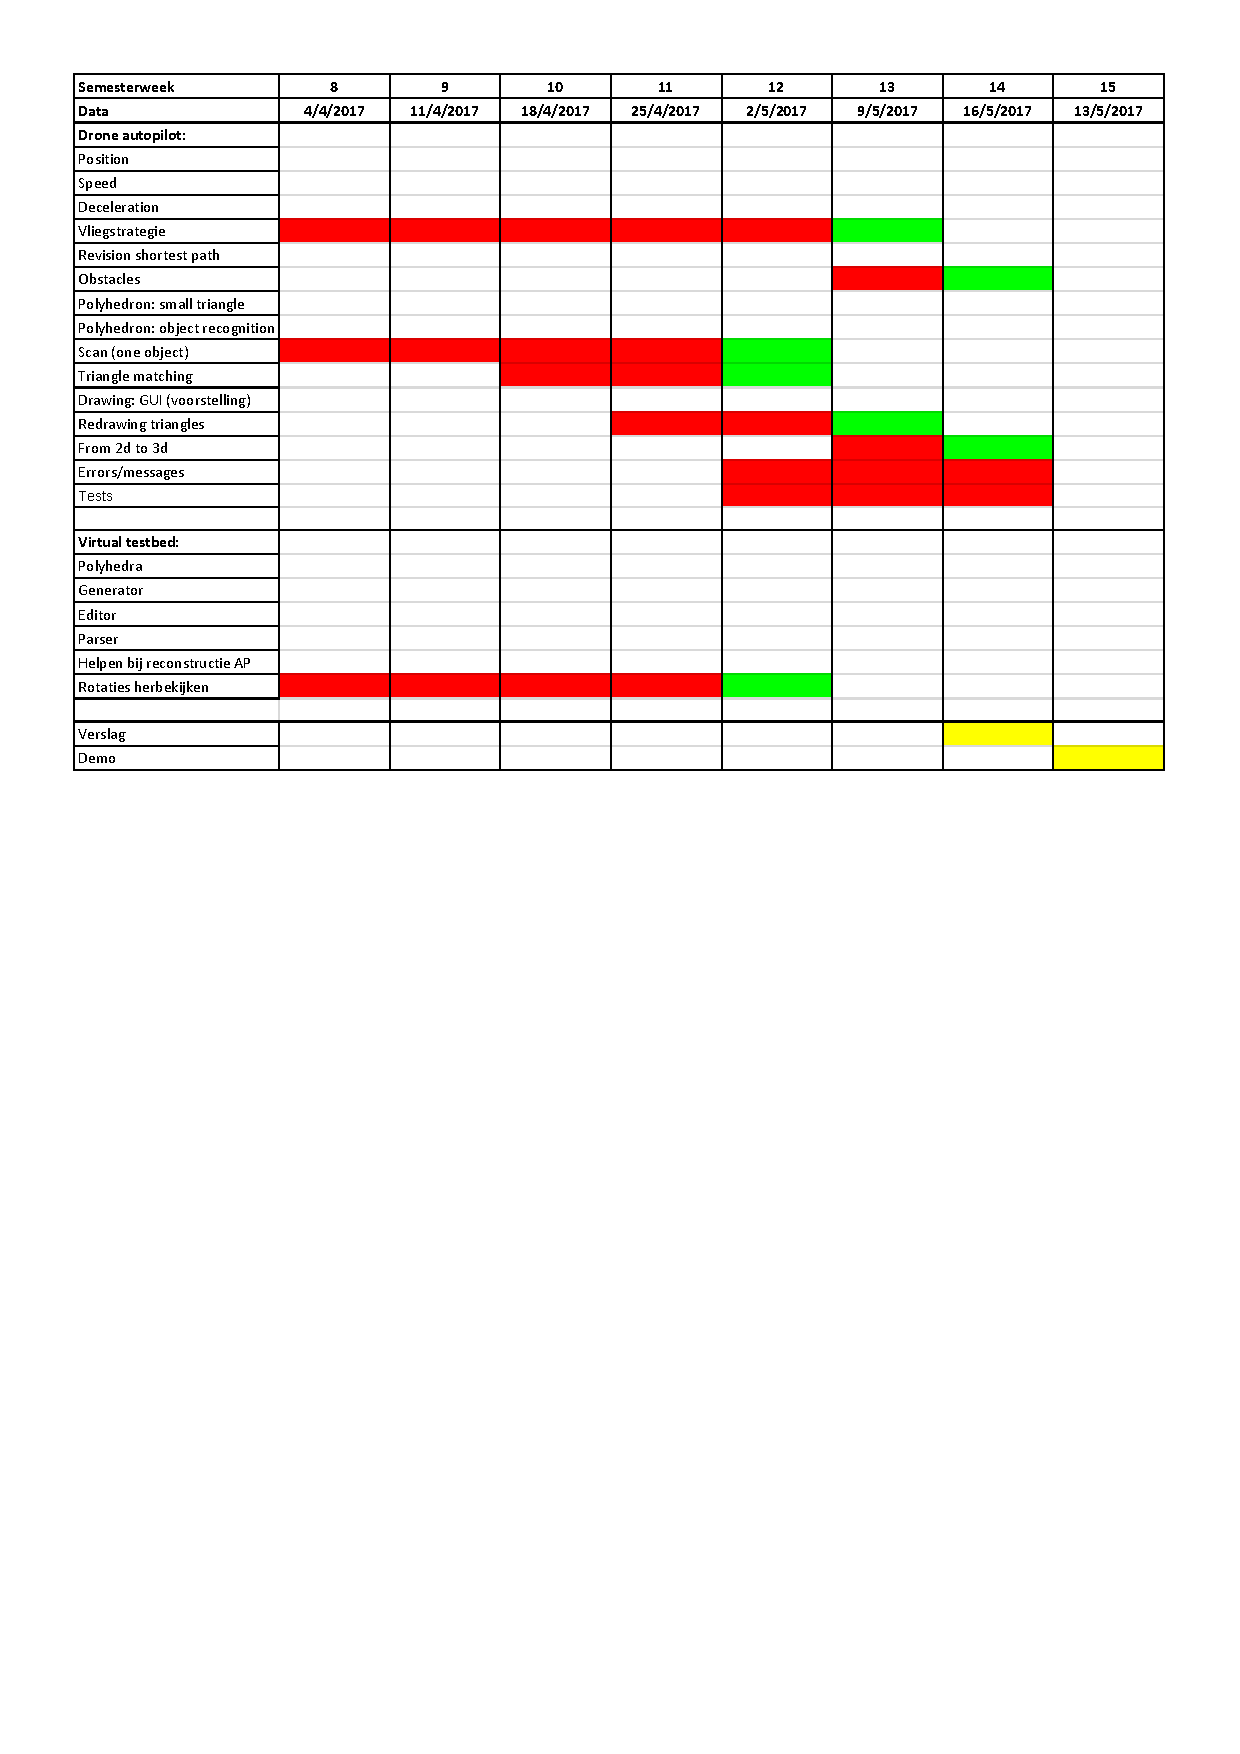
\includegraphics[scale=0.65]{Appendices/Planning_Deel2.pdf}
		\end{center}
		\caption{Deze Gantt chart geeft de planning gedetailleerd weer van het tweede deel. De verschillende delen van de mijlpalen worden opgesplitst om een gedetailleerde taakverdeling te kunnen maken. Ook wordt er tijd voorzien om de tekorten van vorige mijlpalen in te halen. Voltooide onderdelen worden in het groen aangeduid, de deadlines in het geel.}
	\end{figure}

\section{Klassendiagram}
\label{app: Klassendiagram}
\subsection{Virtual Testbed}
\begin{figure}[H]
		\begin{center}
			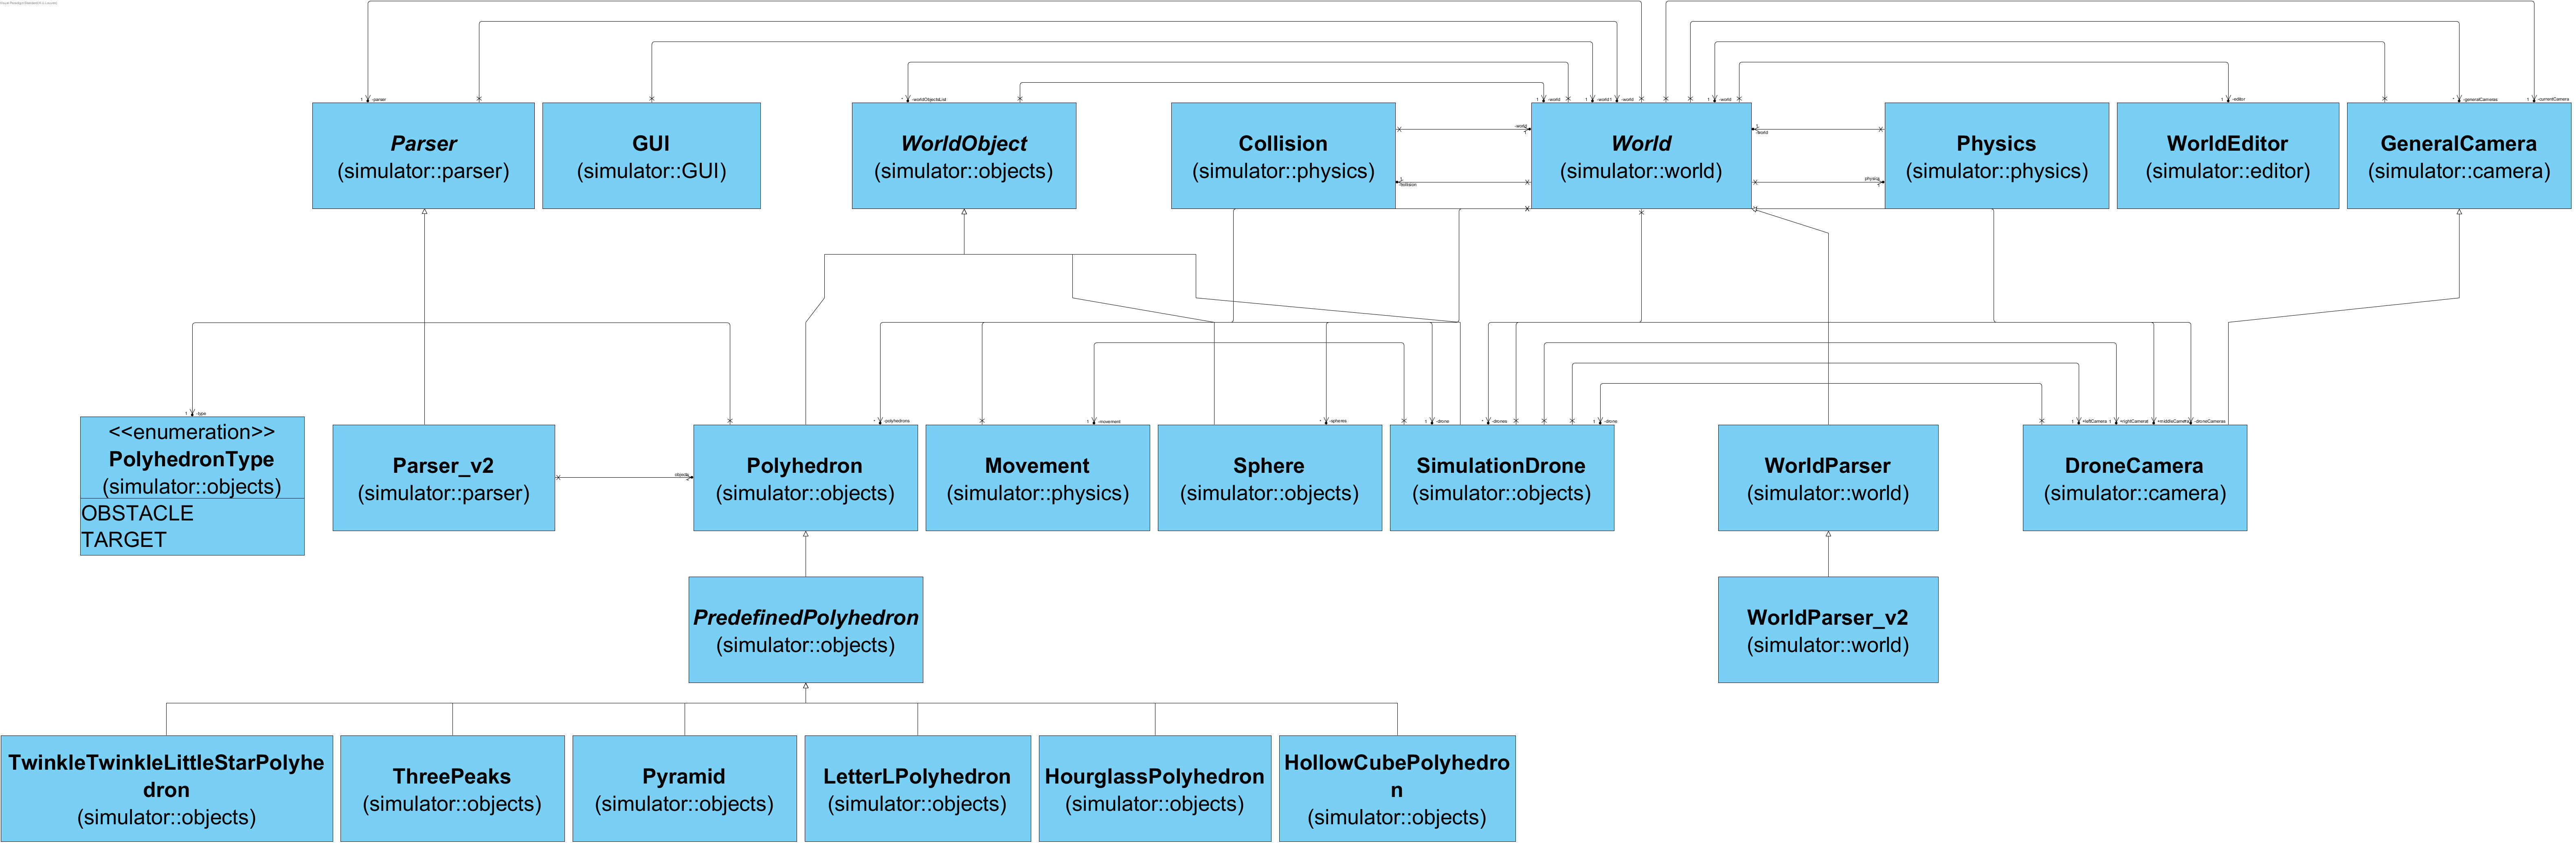
\includegraphics[width=1\linewidth]{Appendices/Simulator.png}
		\end{center}
		\caption{De basisstructuur van het Testbed. Centraal \textit{World}, met de \textit{WorldObjects} (\textit{SimulationDrone}, \textit{Polyhedron}) en enkele hulpklassen. }
\end{figure}
\subsection{Autopilot}
\begin{figure}[H]
		\begin{center}
			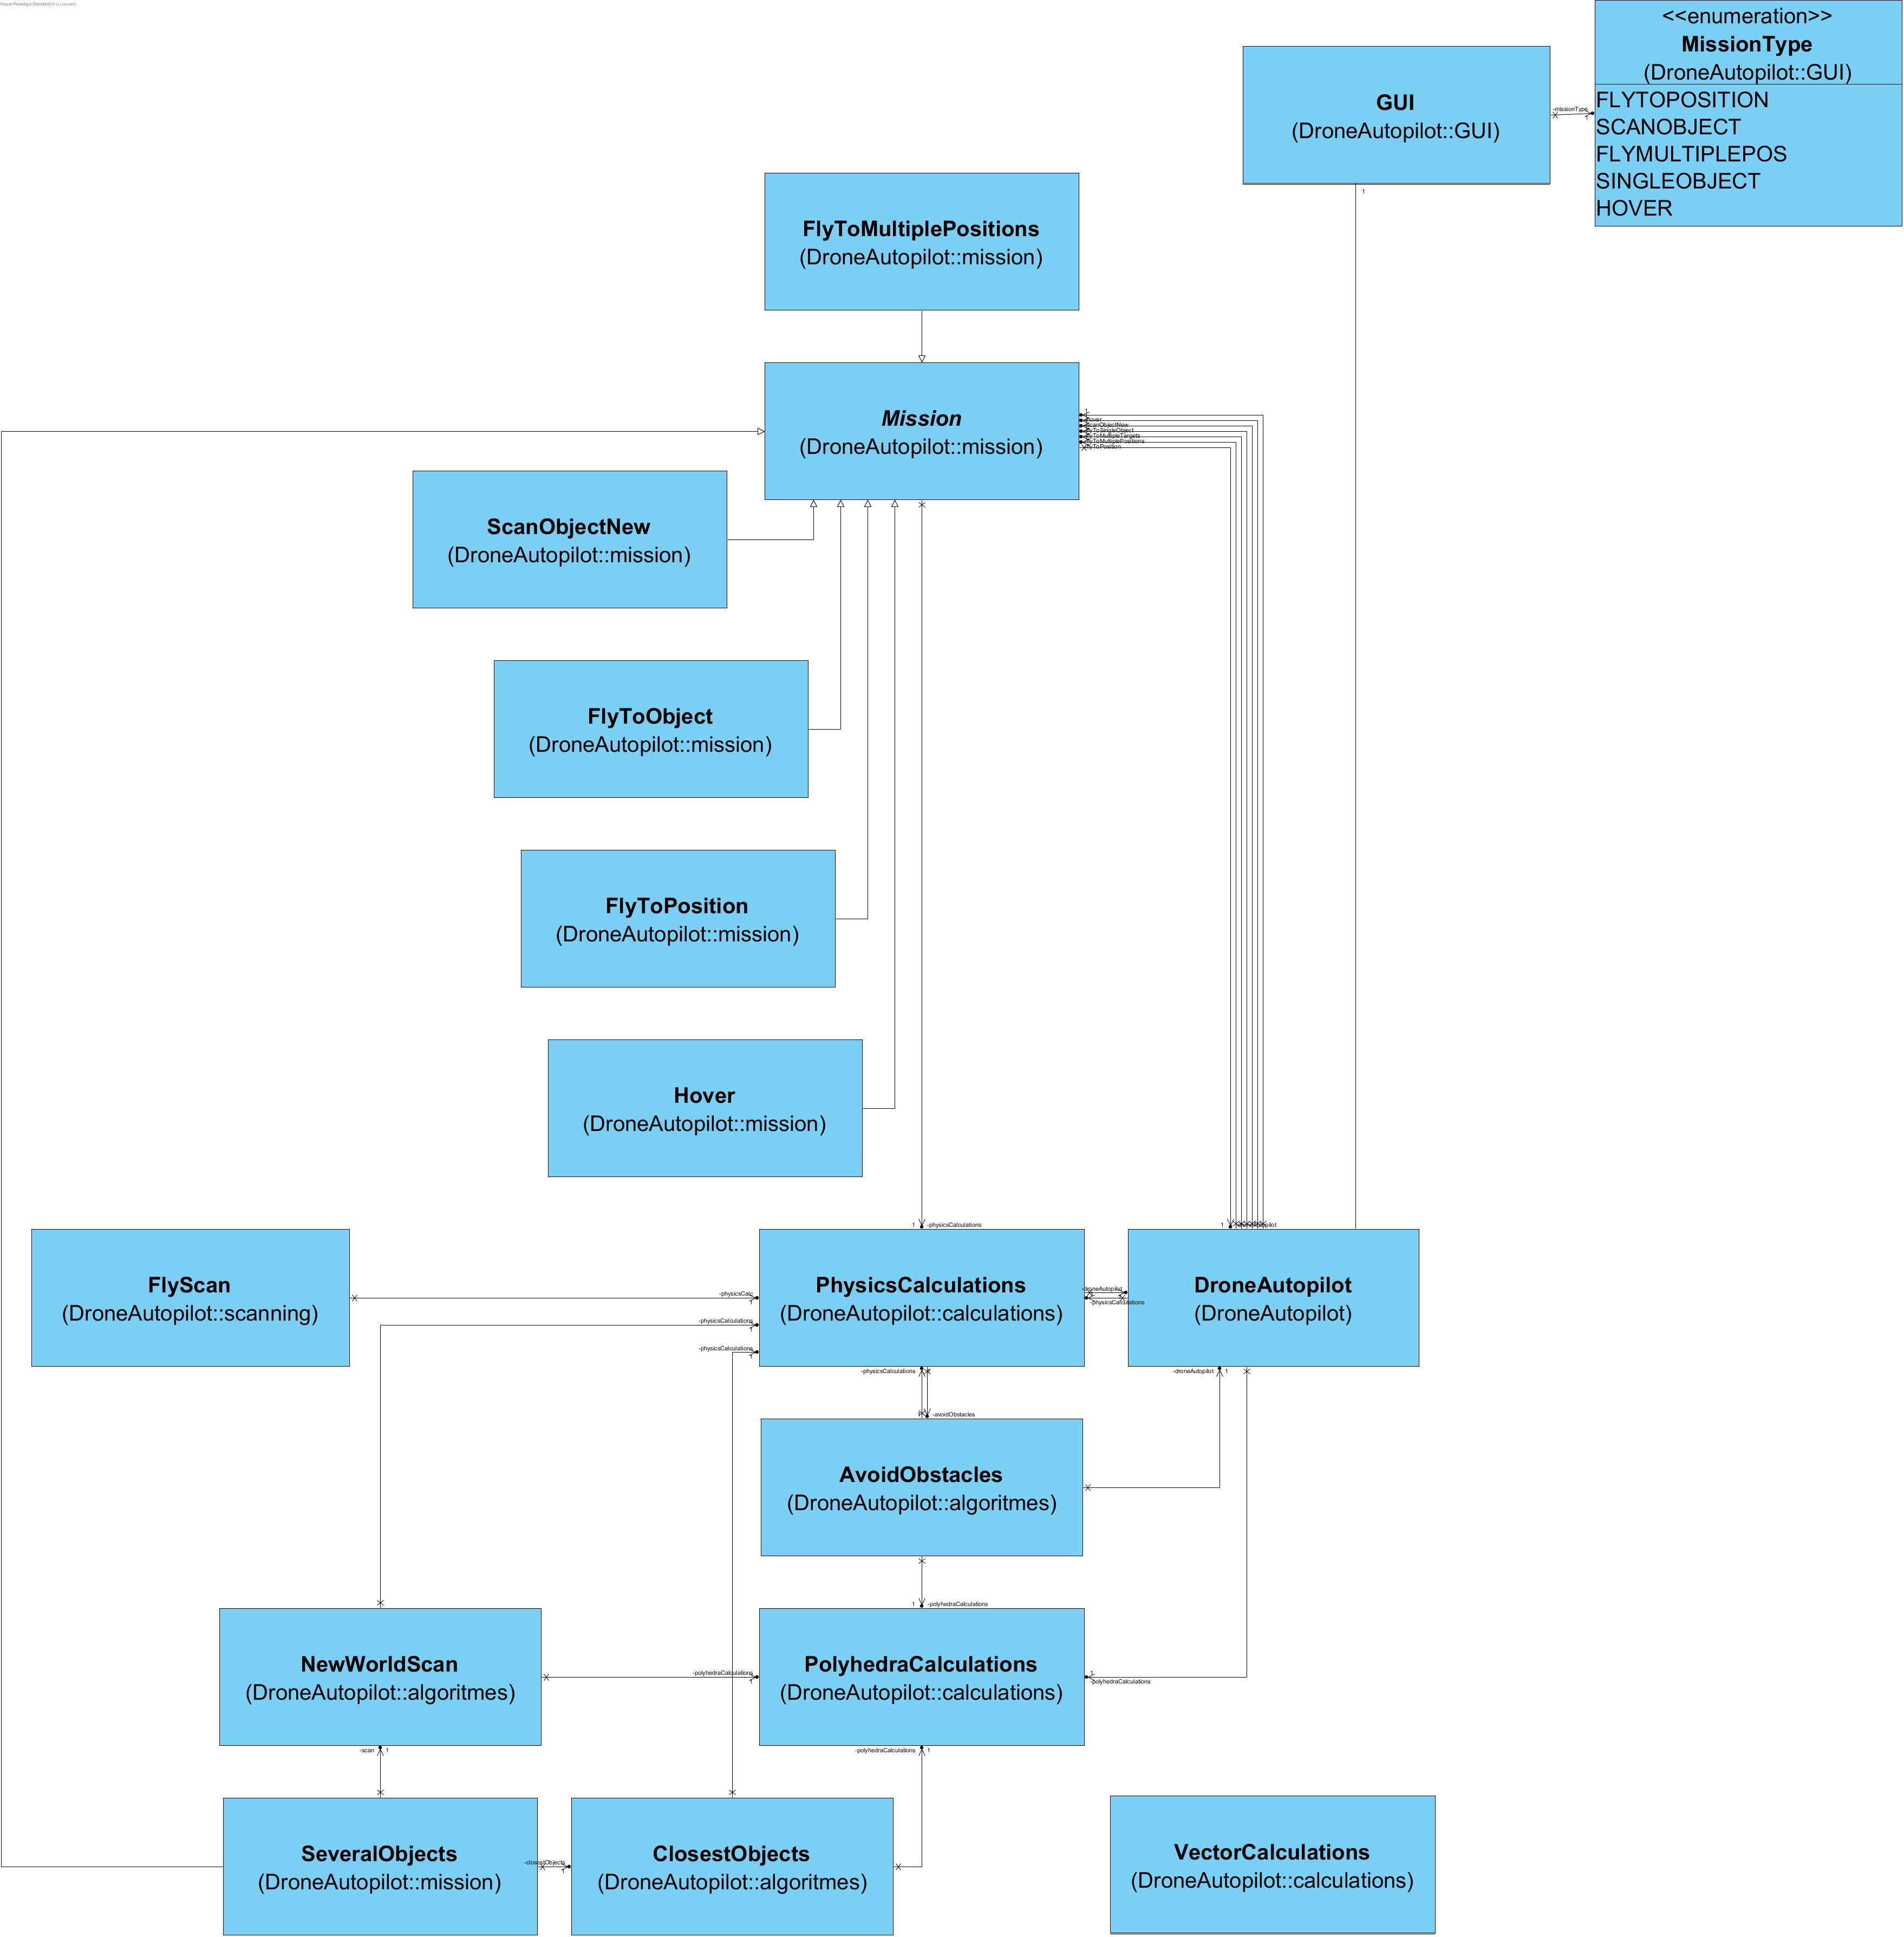
\includegraphics[width=1\linewidth]{Appendices/AP.png}
		\end{center}
		\caption{De basisstructuur weer van de Autopilot. Centrale klassen zijn \textit{Mission, DroneAutopilot} en \textit{PhysicsCalculations}. Dankzij de \textit{Mission}-structuur kon er gemakkelijk opbouwend gewerkt worden en is het duidelijk wat de exacte opdracht van de drone is.}
\end{figure}
\subsection{Scannen}
\begin{figure}[H]
		\begin{center}
			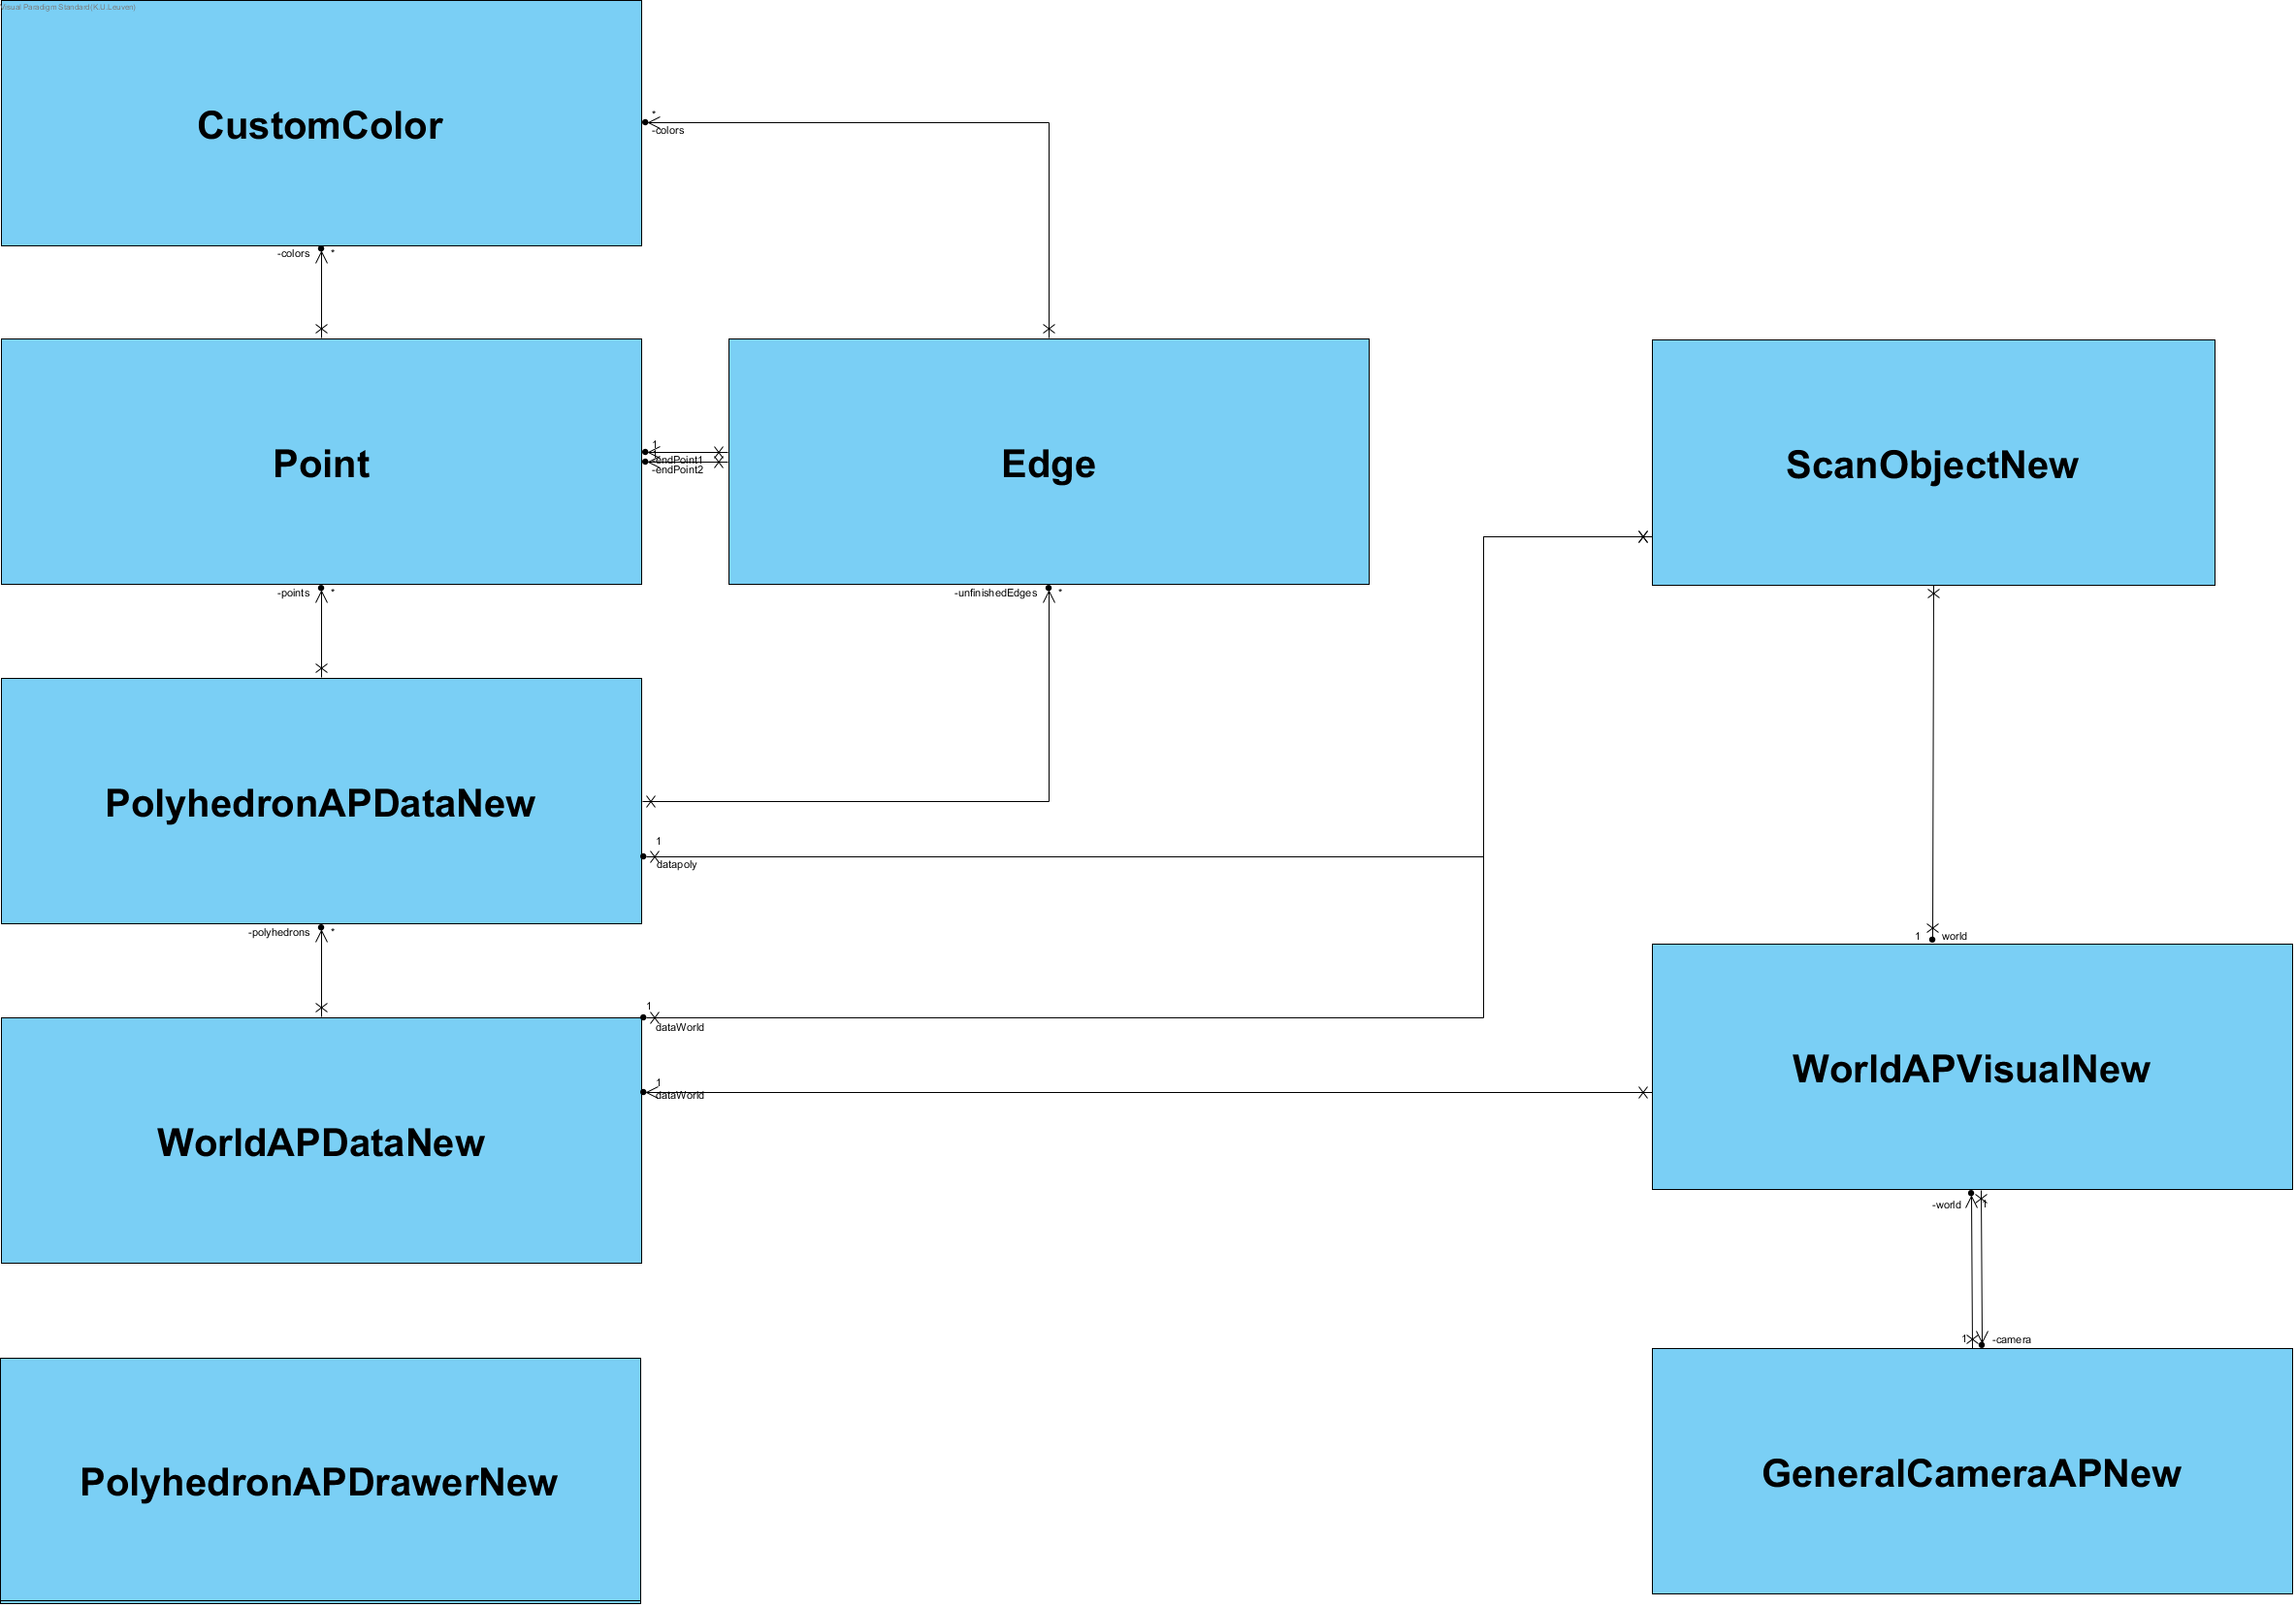
\includegraphics[width=1\linewidth]{Appendices/AP2.png}
		\end{center}
		\caption{De basisstructuur van het scan-gedeelte. Belangrijk zijn de \textit{Polyhedron} en de \textit{WorldAPData} waartoe die behoort. Een \textit{PolyhedronAPData} bestaat uit \textit{Points}, die dan weer \textit{CustomColors} bevatten. }
\end{figure}

% * <arne.vlietinck@gmail.com> 2017-05-09T19:35:45.263Z:
% 
% @Jef: planning/agenda
% Wat waren de moeilijkheden, opgestoken dingen, anders aanpakken (iteratief werken, testbed gemaakt etc.)
% 
% 
% ^.

\end{document}
